Rambøll Tilsyn benytter tre Firebase produkter for at fungere, Authentication(Auth), Realtime Database og Storage.\\

 Firebase Auth\cite{FirebaseAuth} bruges til håndtering af brugere som login og oprettelse. Den indeholder data som e-mail, en hashet password og en unik identifier, der bliver skabt af Firebase Authentication, når brugeren bliver registreret. Firebase tilbyder en Console , som er en hjemmeside, der giver mulighed for at se og manipulere data og konfigurere sin Firebase. På Figur \ref{fig:FirebaseAuthPNG} kan en oversigt med informationer over brugere ses. 
\begin{figure}[H] % (alternativt [H])
	\centering
	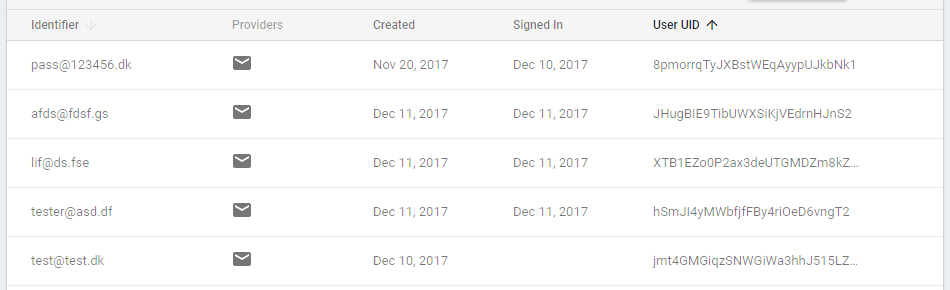
\includegraphics[height=5cm, width=15cm]{../ArkitekturDesign/Design/Firebase/FirebaseAuth.PNG}
	\caption{Oversigt over authentication data i Firebase Console.}
	\label{fig:FirebaseAuthPNG}
\end{figure}

Firebase Realtime Database bliver i forbindelse med applikationen brugt som en platform til at indeholde og give et simpelt overblik over informationen, der er gemt i databasen, som vist på Figur \ref{fig:FirebaseDBPNG}.  
 
\begin{figure}[H] % (alternativt [H])
	\centering
	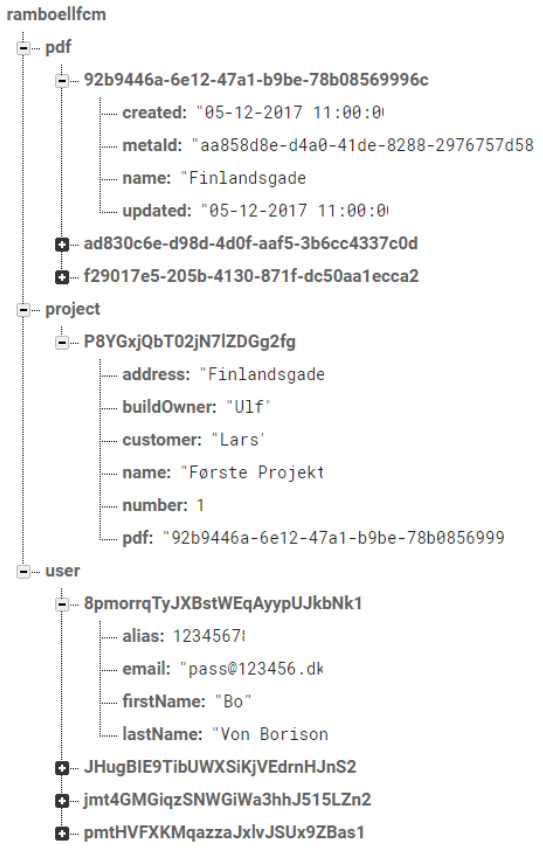
\includegraphics[height=10cm, width=8cm]{../ArkitekturDesign/Design/Firebase/FirebaseDB.PNG}
	\caption{Oversigt over databasen i Firebase Console.}
	\label{fig:FirebaseDBPNG}
\end{figure}

På Figur \ref{fig:FirebaseDBPNG}, ses hvordan applikationens database er struktureret som et træ med en root node\cite{rootNode}, der hedder ramboellfcm og som derfra bliver opdelt i 3 noder:
\textbf{pdf}, \textbf{project} og \textbf{user}.\\

\textbf{Pdf}-node indeholder en liste af Guid \cite{GUID}, som er keys til en pdf-node og som bruges til at tilgå de specifikke pdf-noder. Under hver specifik pdf node er der 4 key-value-pair\cite{KVP}. Disse keys fungerer også som en reference til Firebase Storage, når det bliver nødvendigt at hente PDF filen ned lokalt.

Dette gør, at man kan se, hvilke projekter og pdf'er der findes i databasen og afvente med at downloade PDF'en, indtil man har brug for den. På den måde kan man få en oversigt over, hvilket projekter og pdf'er der er og kun hente de data, man har behov for. 
\begin{itemize}
	\item \textbf{created}\\
	Giver en dato for, hvornår objektet er oprettet med en nøjagtighed i sekunder, der kan ændres, hvis det føles nødvendigt.\\
	\item \textbf{metaId}\\
	En referrence til JSON-filen der er gemt i Firebase Storage\cite{FirebaseStorage}, som indeholder de objekter, der skal tegnes på pdf'en. Disse bliver brugt, når der skal indlæses nye objekter, der bliver oprettet på pdf'en.\\ 
	
	\item \textbf{name}\\
	Navnet på PDF'en som er skrevet i klar tekst og indtastet af brugeren. En guid vil ikke give meget mening for brugeren.\\
	
	\item \textbf{updated}\\
	En timestamp der fortæller hvornår JSON-filen, som meta-filen refererer til, sidst er blevet ændret. Dette bruger applikationen til at sammenligne den lokale version af JSON-filen med den, der ligger i Storage.   
\end{itemize}

	\textbf{Project-node} har den samme structur som \textbf{pdf-node} af samme grund. Der er i stedet for 6 key-value-pair. 
	\begin{itemize}
		\item  \textbf{address}\\
		Værdien gemt i address vil være et vejnavn, der fortæller, hvor projektet befinder sig.\\
		\item  \textbf{customer}\\
		Denne key indeholder kontaktinformationerne for, hvem der udføres tilsynsrapporter for.\\
		\item  \textbf{name}\\
		Værdien gemt i name vil være navnet på projeket.\\
		\item  \textbf{number}\\
		Rambøll bruger et projektnummer til alle deres projekter. Dette indsætter de selv som brugere og derfor gemmes denne information her\\
		\item  \textbf{pdf}\\
		En reference til en pdf-node, samt en reference til Firebase Storage så applikationen kan downloade PDF'en, når den først har brug for det.\\
	\end{itemize}

\textbf{User} node indeholder brugerdefineret data, der tilhører brugerne af applikationen. Det id der bliver brugt som key til user stammer fra Firebase Authentication og er en reference til User guid, som ses på Figur \ref{fig:FirebaseAuthPNG}. 
\begin{itemize}
	\item \textbf{alias} \\
	Her gemmes telefonnummeret til brugeren. \\
	\item \textbf{email} \\
	Brugerens e-mail vil blive gemt i både Firebase- Authentication og Storage for at gøre det let tilgænglig at tilgå.\\
	\item \textbf{firstName} \\
	Fornavnet på brugeren.\\
	\item \textbf{firstName} \\
	Efternavnet på brugeren.\\

\end{itemize}

\clearpage

